\documentclass[final]{beamer}

% ====================
% Packages
% ====================

\usepackage[T1]{fontenc}
\usepackage{lmodern}
\usepackage[size=custom,width=120,height=72,scale=1.0]{beamerposter}
\usetheme{gemini}
\usecolortheme{gemini}
\usepackage{graphicx}
\usepackage{booktabs}
\usepackage{tikz}
\usepackage{xcolor}
\usepackage{pgfplots}
\pgfplotsset{compat=1.7}

% ====================
% Lengths
% ====================

% If you have N columns, choose \sepwidth and \colwidth such that
% (N+1)*\sepwidth + N*\colwidth = \paperwidth
\newlength{\sepwidth}
\newlength{\colwidth}
\setlength{\sepwidth}{0.025\paperwidth}
\setlength{\colwidth}{0.3\paperwidth}

\newcommand{\separatorcolumn}{\begin{column}{\sepwidth}\end{column}}

% ====================
% Title
% ====================

\title{DESCRIBING THE WOBBLING MOTION IN \texorpdfstring{$^{163}$}{163}Lu THROUGH A SEMI-CLASSICAL APPROACH}

\author{Robert Poenaru \inst{1,2} | \texttt{robert.poenaru@protonmail.ch}}

%\institute[shortinst]{\inst{1} Doctoral School of Physics, University of Bucharest, Bucharest, Romania \samelineand \inst{2} Department of Theoretical Physics, Horia-Hulubei National Institute of Nuclear Physics and Engineering, Bucharest-Magurele, Romania}

\institute[shortinst]{\inst{1} Doctoral School of Physics, University of Bucharest, Bucharest, Romania \\ \inst{2} Department of Theoretical Physics, Horia-Hulubei National Institute of Nuclear Physics and Engineering, Bucharest-Magurele, Romania}

% ====================
% Body
% ====================

\begin{document}

\addtobeamertemplate{headline}{} 
{\begin{tikzpicture}[remember picture, overlay]
     \node [anchor=north east, inner sep=0.9cm]  at (current page.north east)
     {
\includegraphics[height=10cm]{./images/logos/logo.png}};
     \node [anchor=north west, inner sep=0.9cm]  at (current page.north west)
     {
\includegraphics[height=9cm]{./images/logos/uniLogo.png}};
  \end{tikzpicture}}
  
\begin{frame}[t]
\begin{columns}[t]
\separatorcolumn
\begin{column}{\colwidth}
  \begin{block}{Introduction}
Wobbling Motion (WM) is a unique feature of triaxial nuclei. These systems have strong (charge) + (mass) + (shape) deformations and asymmetries that are stable in the ground state.

\textbf{Current project goal:} Describe the wobbling spectrum of an odd-A nucleus, i.e., $^{163}$Lu by using a semi-classical set of equations for the system's dynamics.
\heading{Wobbling Motion in Nuclei}
  WM employs a \emph{precession} of the total angular momentum $\vec{I}$ combined with an \emph{oscillation} of its projection on the rotational axis. Different \emph{core-particle} couplings lead to different wobbling regimes.
  \begin{figure}
      \centering
     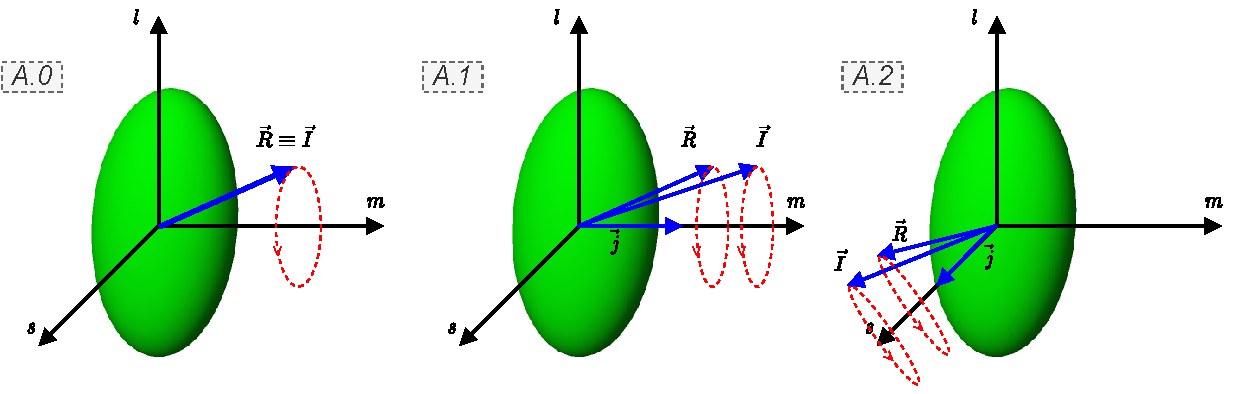
\includegraphics[scale=1.5]{images/wobbling_Regimes_COUPLING_SCHEME.pdf}
      \caption{An illustration with the wobbling regimes which can occur in a nucleus. From left to right: \emph{simple/ideal wobbler}, \emph{longitudinal wobbler}, \emph{transverse wobbler}.}
      \label{wobbling-regimes}
  \end{figure}
  \begin{figure}
      \centering
     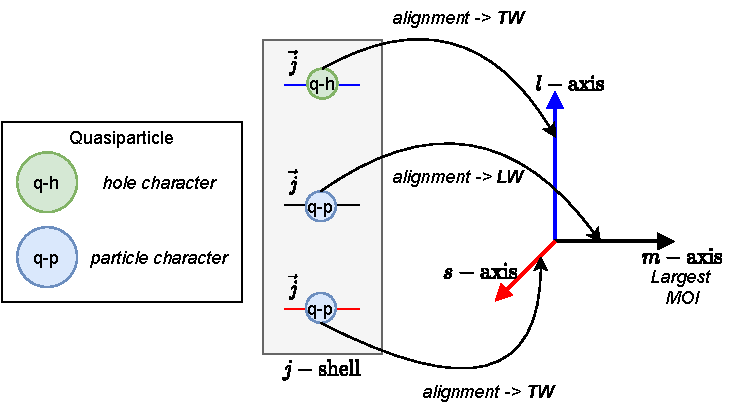
\includegraphics[scale=2.3]{images/wobbling_Regimes_updated.pdf}
      \caption{\textbf{Longitudinal} (LW) and \textbf{Transverse} (TW) Wobbling regimes, depending on the \emph{core-particle} coupling. $l,m,s$ are the principal axes of a triaxial ellipsoid.}
      \label{tw-lw-wobbling}
  \end{figure}
  \end{block}
\end{column}
\separatorcolumn
\begin{column}{\colwidth}
  \begin{block}{Wobbling Motion: Odd-A Formalism}
The system is described by the total Particle-Rotor-Model Hamiltonian:
\begin{align}
    \hat{H}=\hat{H}_\text{core}+\hat{H}_\text{sp}\ ,
\end{align}
where $\hat{H}_\text{core}$ describes the triaxial core, and $\hat{H}_\text{s.p.}$ is the single-particle potential that corresponds to the odd nucleon (for $^{163}$Lu it is the $\vec{j}=\pi(i_{13/2})$ nucleon).

Hamiltonian is dequantized through the \textbf{Time Dependent Variational Principle} and a set of \emph{classical} expressions for the system dynamics are obtained.
\begin{align}
    \mathcal{H}_\text{classical}=\mathcal{H}_\text{min}+{\color{red}\Omega_1}\left(n_{w1}+\frac{1}{2}\right)+{\color{blue}\Omega_2}\left(n_{w2}+\frac{1}{2}\right)\ .
\end{align}
The system's behavior consists of a main rotational motion due to the core ($\mathcal{H}_\text{min}$), and two harmonic-like motions emerging from the core-particle coupling ($\Omega_1$ and $\Omega_2$).
  \end{block}
    \begin{block}{Results}
    The excitation energies for each wobbling band (triaxial strongly-deformed -TSD- band) were obtained using the above equation.
  \begin{figure}
\centering
\begin{minipage}{.5\textwidth}
  \centering
  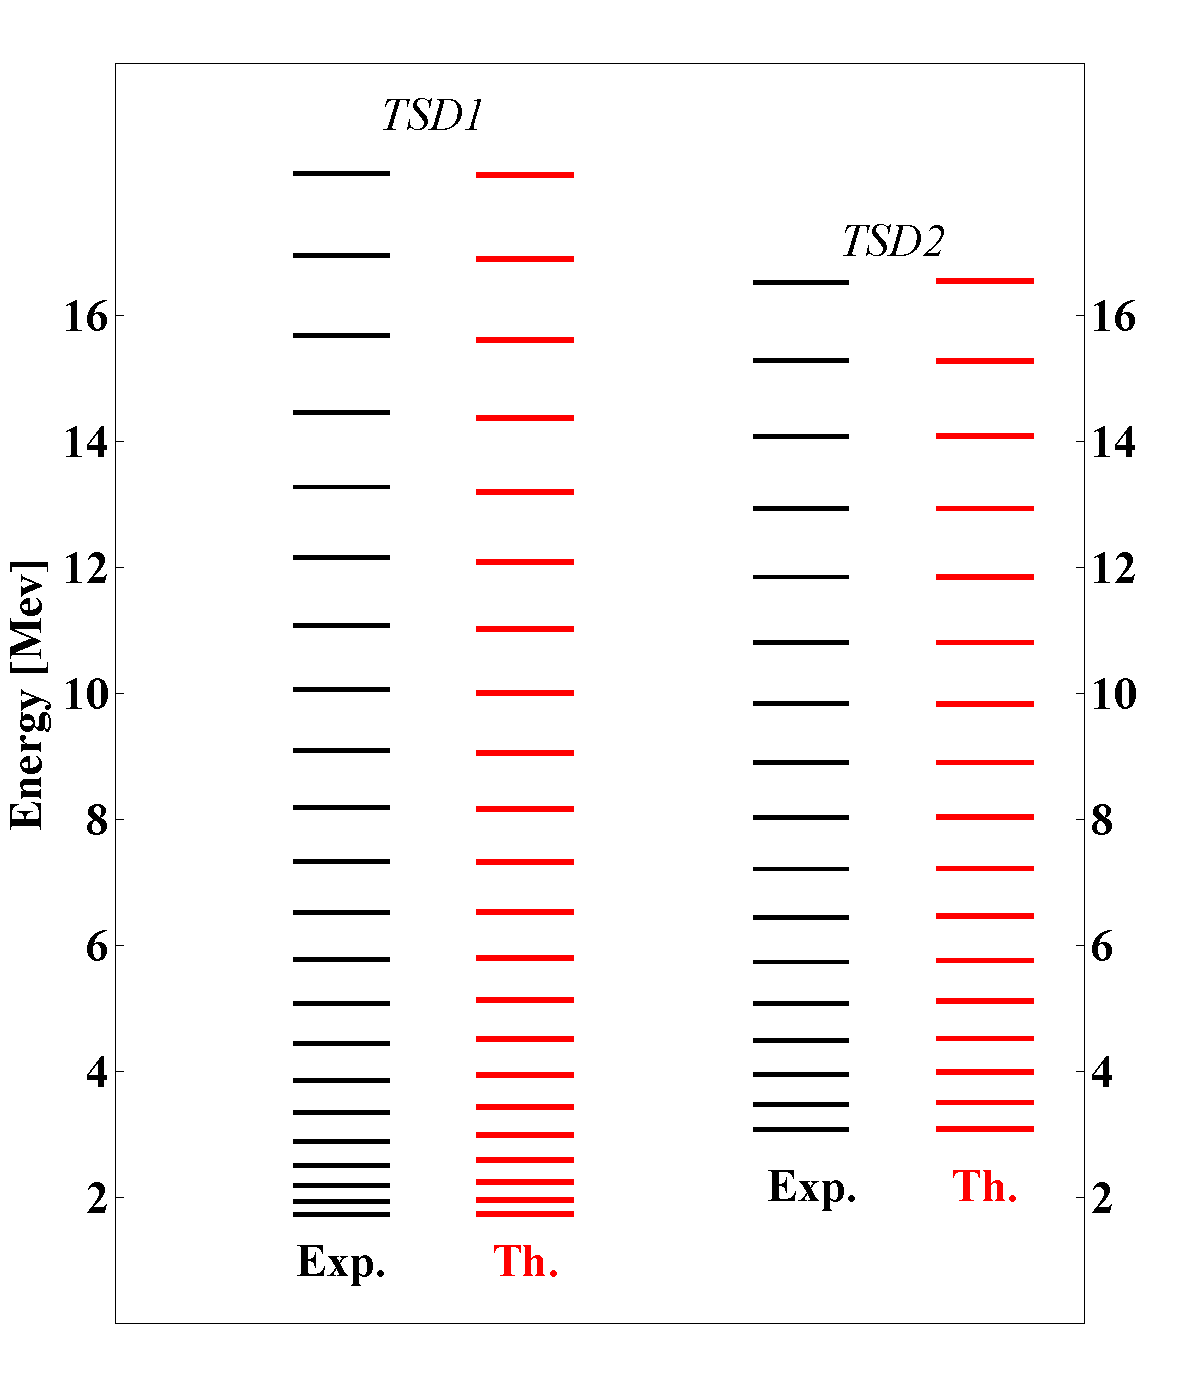
\includegraphics[scale=0.9]{images/TSD-12.pdf}
\end{minipage}%
\begin{minipage}{.5\textwidth}
  \centering
 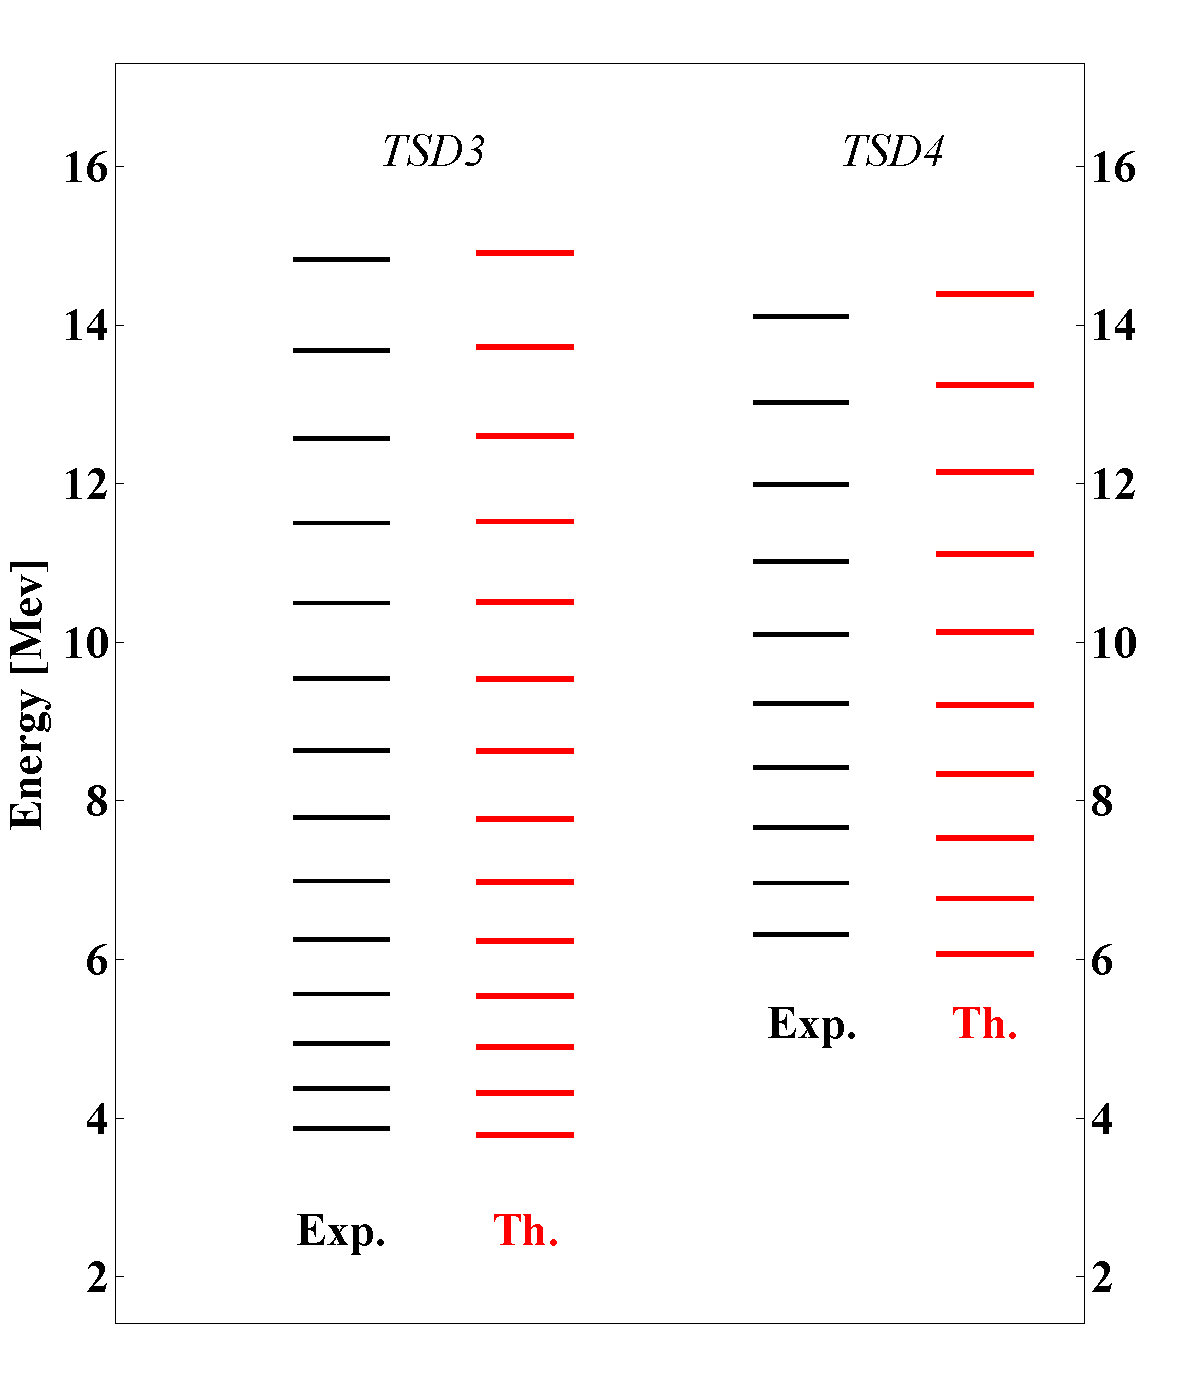
\includegraphics[scale=0.9]{images/TSD-34.pdf}
\end{minipage}
\caption{Energy spectrum of the four triaxial strongly-deformed bands in $^{163}$Lu.}
    \label{tsd-bands}
\end{figure}

  \end{block}
\end{column}
\separatorcolumn
\begin{column}{\colwidth}
  \begin{figure}
\centering
\begin{minipage}{.5\textwidth}
  \centering
  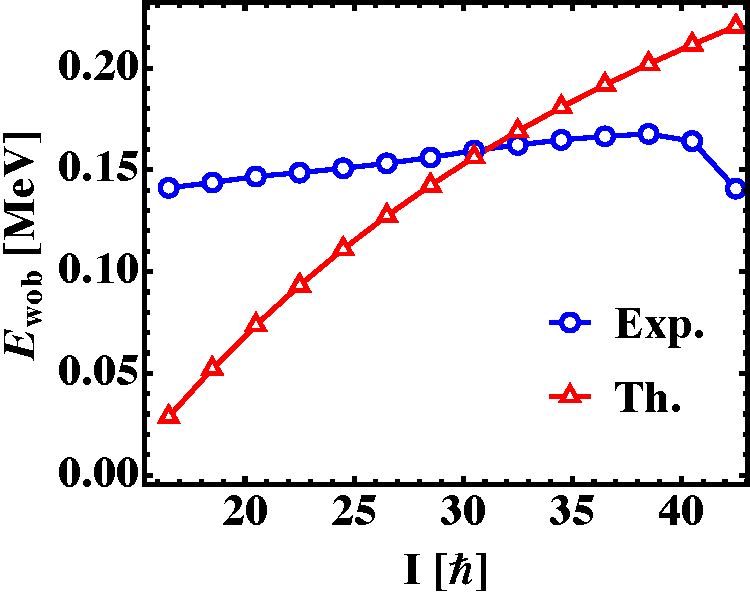
\includegraphics[scale=1.27]{images/wobbEnergies.pdf}
\end{minipage}%
\begin{minipage}{.5\textwidth}
  \centering
 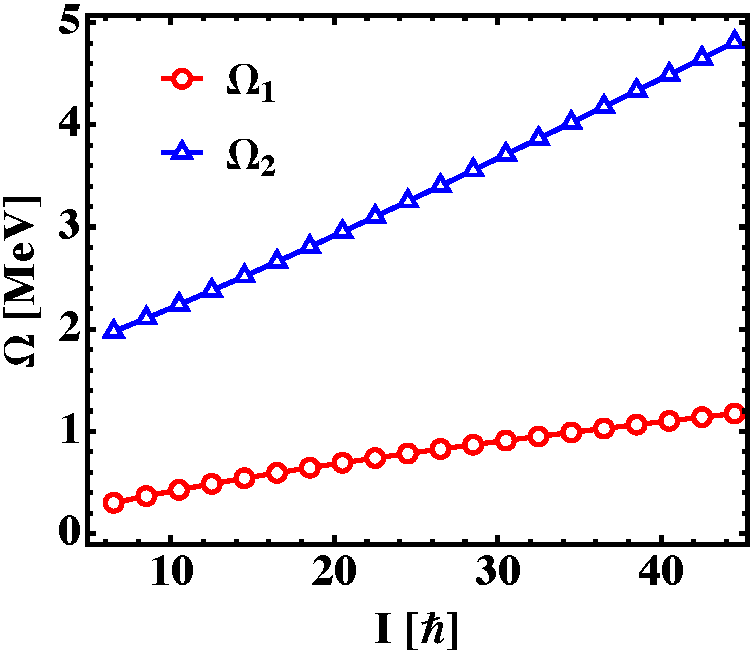
\includegraphics[scale=1.2]{images/wobbFrequencies.pdf}
\end{minipage}
\caption{\textbf{Left:} The wobbling energies, defined as the $E_\text{wob}=E_1(I)-\frac{1}{2}(E_0(I+1)-E_0(I-1))$, where $E_0$ is the ground-state band and $E_1$ is the first excited band. \textbf{Right:} The wobbling frequencies obtained analytically after the dequantization of $\hat{H}$. $\Omega_1$ corresponds to the motion of core, while $\Omega_2$ corresponds to the dynamics of the odd-nucleon.}
    \label{wobb-energies}
\end{figure}
\begin{figure}
\centering
\begin{minipage}{.65\textwidth}
  \centering
  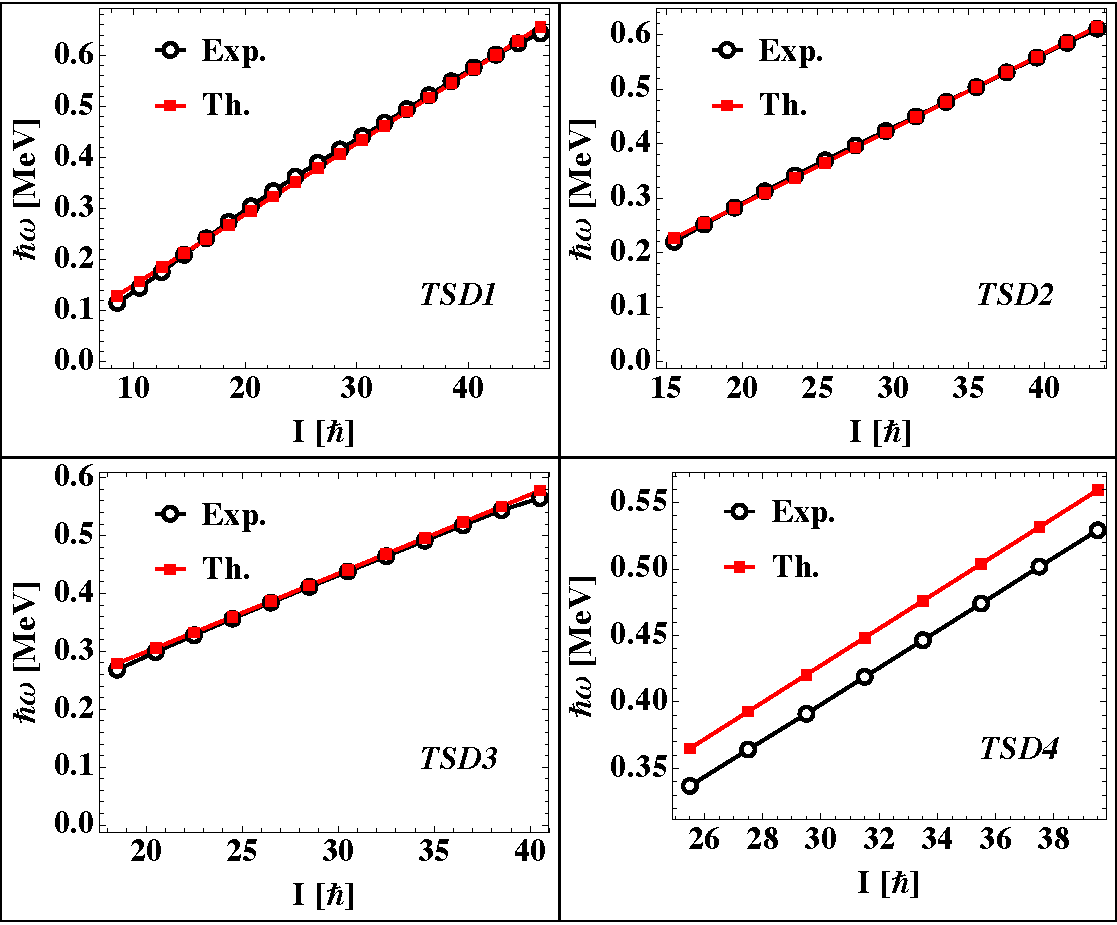
\includegraphics[scale=1.1]{images/rotFreqs.pdf}
\end{minipage}%
\begin{minipage}{.35\textwidth}
  \centering
 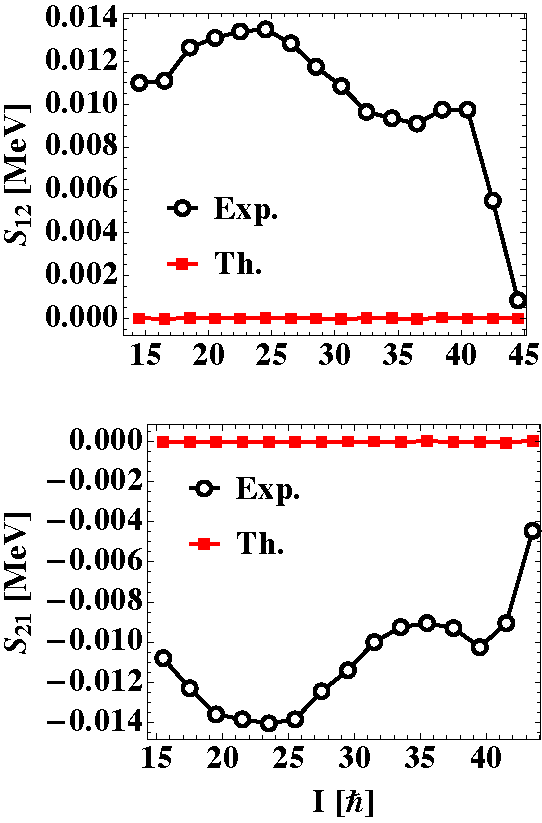
\includegraphics[scale=1.2]{images/staggers.pdf}
\end{minipage}
    \caption{\textbf{Left:} The rotational frequencies of $^{163}$Lu, defined as the averaged increase in energy between two wobbling states with respect to the increase in angular momentum of the total system. \textbf{Right:} Energy staggering between the bands TSD1 and TSD2.}
    \label{rotational-freqs}
\end{figure}
    \begin{block}{Conclusions}
\begin{itemize}
    \item The excitation spectrum of the wobbling states in $^{163}$Lu is accurately described by a classical set of equations.
    \item The single-particle motion has a larger contribution in the total energy of a wobbling nucleus (Fig. \ref{wobb-energies}).
    \item Due to the increasing trend of the wobbling energies (Fig. \ref{wobb-energies} left), the nucleus has a longitudinal wobbling regime.
\end{itemize}
  \end{block}
\end{column}
\separatorcolumn
\end{columns}
\end{frame}

\end{document}